\documentclass{article}
\usepackage[utf8]{inputenc}
\usepackage{graphicx}
\usepackage{sectsty}


\title{Final Report}
\author{Group 4: Pico Bello B.V.}
\date{22-01-2015}
\setcounter{tocdepth}{2}




\begin{document}
	\fontencoding{T1}\fontfamily{lmss}\fontseries{m}\selectfont

	\allsectionsfont{\fontfamily{lmss}\selectfont}


	\maketitle
	\begin{figure}[ht!]
		\centering
		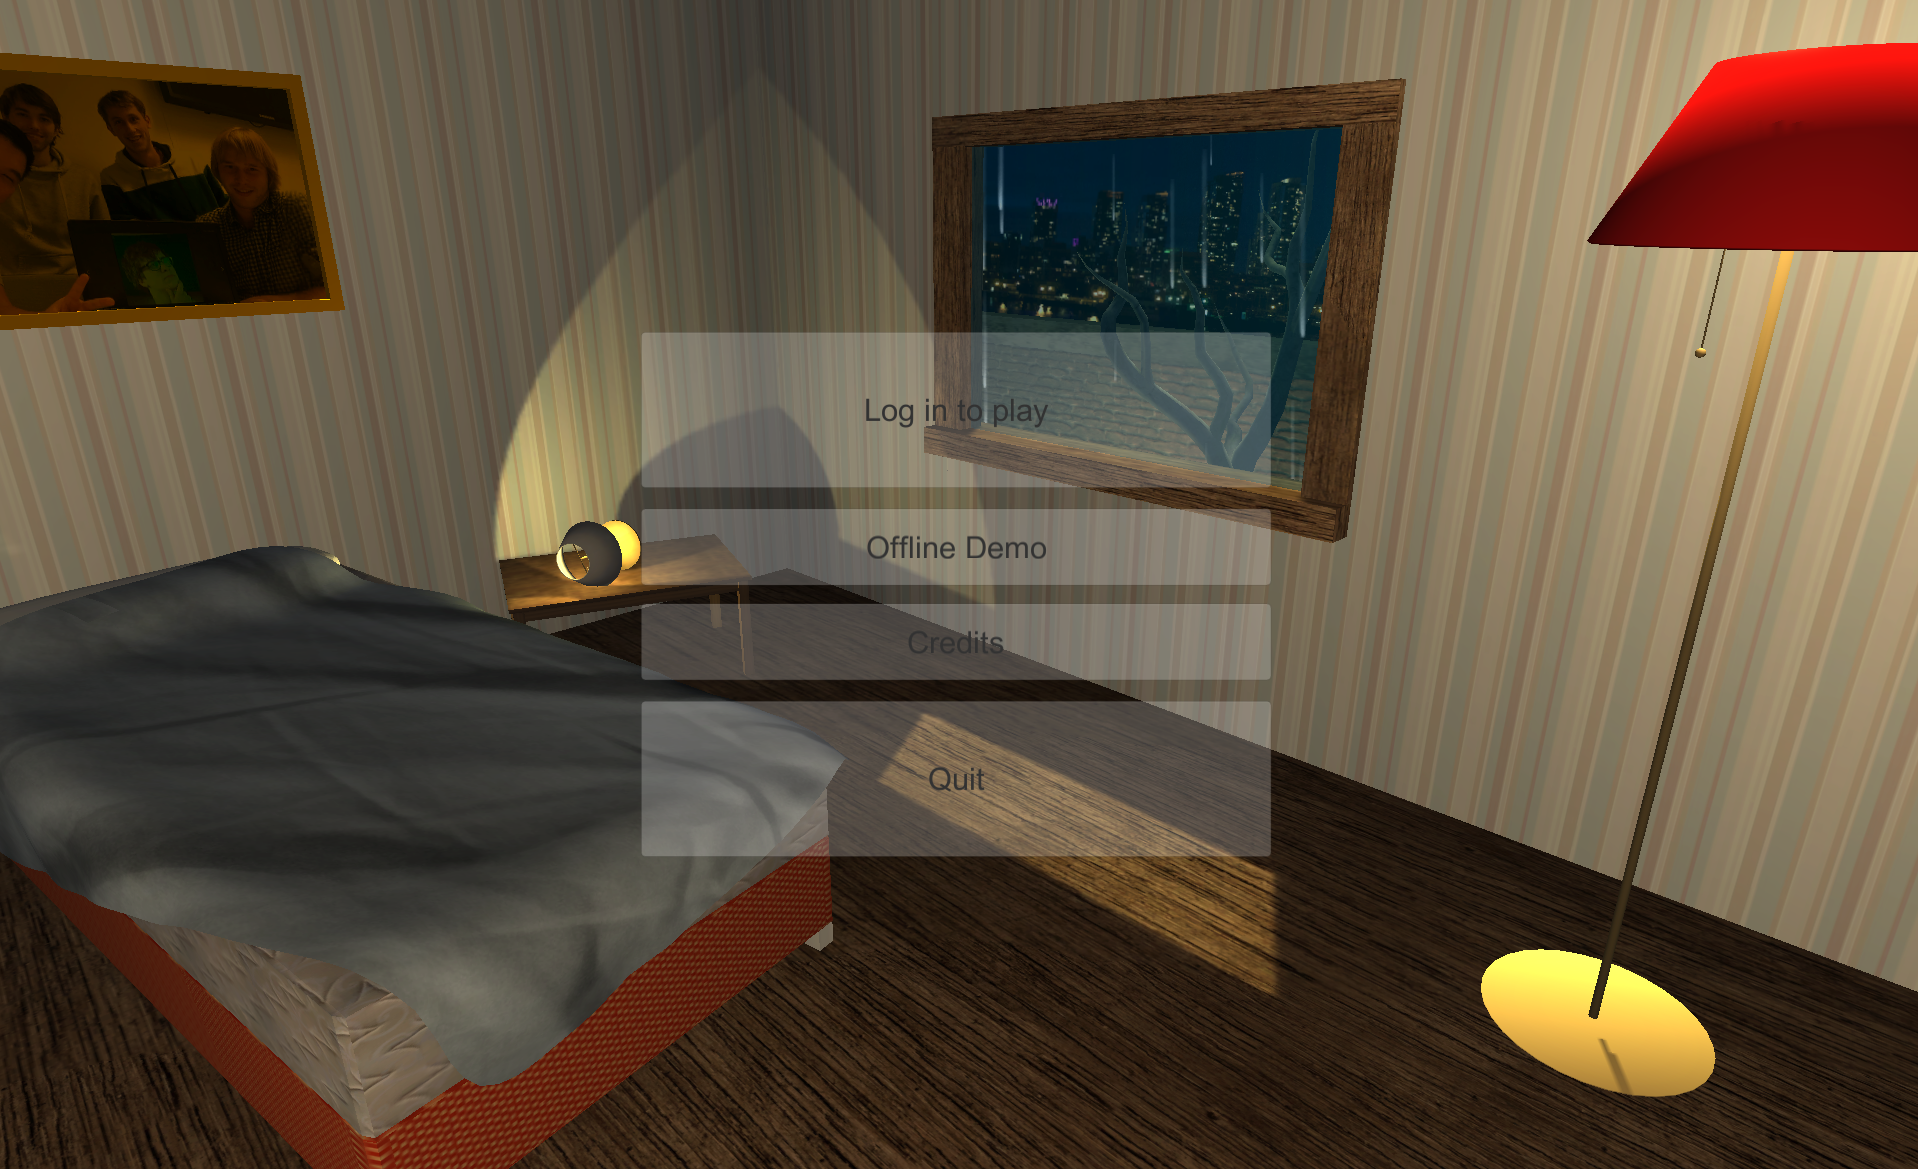
\includegraphics[width=120mm]{images/Front.png}
	\end{figure}
	\newpage
\subsection*{Project Name}
	\qquad Awesome Spel
\subsection*{Team Name}
	\qquad Group 4: Pico Bello B.V.
\subsection*{Team Members}
	\begin{itemize}
		\item\textbf{Thomas de Boer}, Game Designer.\\Mechanical Engineering, 3mE. 4172760 - t.w.j.deboer@student.tudelft.nl\\
		\item\textbf{Luuk de Niet}, Lead Artist.\\Applied Sciences, TN. 4139658 - l.f.deniet93@gmail.com\\
		\item\textbf{Boyd Verdoorn}, Lead Programmer.\\Applied Sciences, TN. 4209346 - b.c.verdoorn@student.tudelft.nl\\
		\item\textbf{Rense Wisse}, World Builder.\\Civil Engineering, CiTG. 4230027 - r.r.wisse@student.tudelft.nl\\
		\item\textbf{Jesper Spillenaar Bilgen}, Producer.\\Mechanical Engineering, 3mE. 4147405 - jesper\_sb\_91@hotmail.com
	\end{itemize}

	\begin{figure}[ht!]
		\centering
		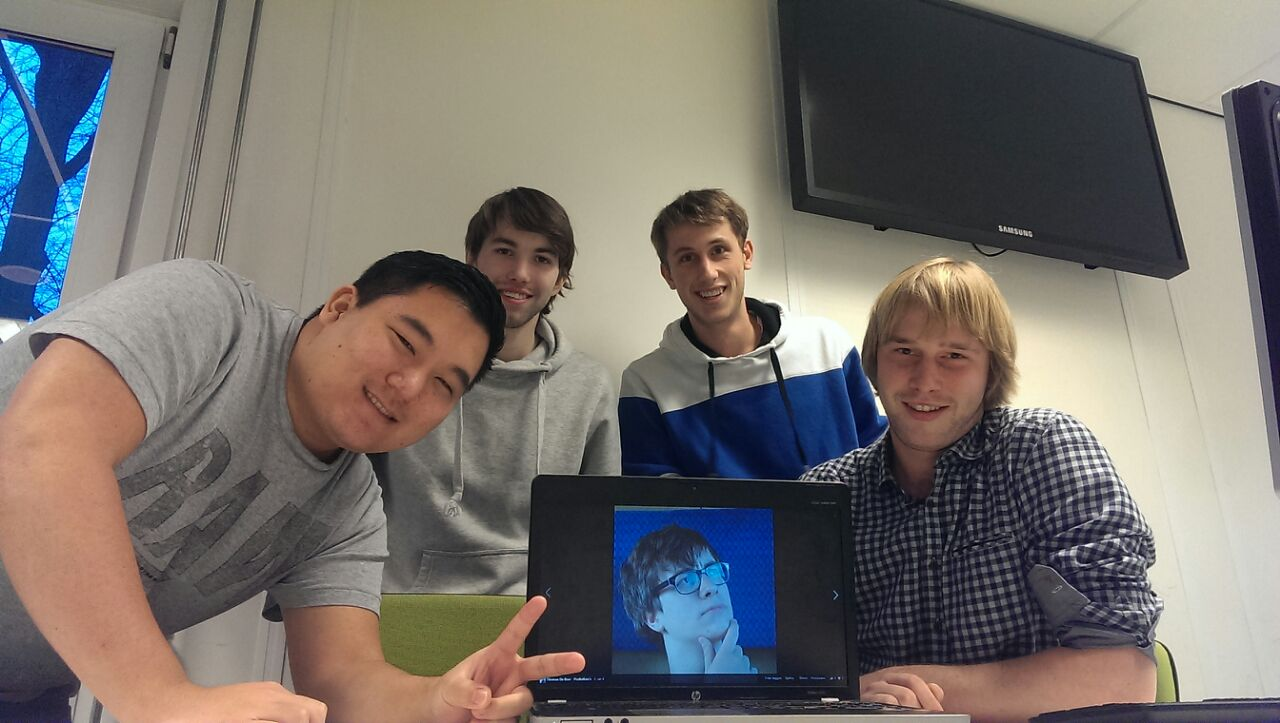
\includegraphics[width=100mm]{images/Team.jpg}
		\caption{From left to right: Boyd, Rense, Thomas (on laptop), Jesper and Luuk}
		\end{figure}

	\newpage
		\tableofcontents
	\newpage

\section{Introduction}
	Awesome Spel is a game that is based around the old Film Noir movie genre, but with a modern twist. The game will be in color, albeit a bit grimey. The player should solve a hideous murder, while playing as a detective, George Carter. There are several ways to collect evidence, by searching for clues, interrogation and exploration.

	\subsection{How and Why?}
		This game is being developed as part of an assignment for the TU Delft in the Netherlands. We are required to use Unity 4.6 and Blender as development tools. Other tools we use are Crazybump, for creating bump maps, audacity as a audio suite and LaTeX for Deliverables. The teams for the assignment were put together based on experience in different fields. We don't have any team members with a design background, so this is a small hurdle. We try to overcome this by working on the models with a large part of the team.

	\subsection{Inspiration}
		Our Inspiration was games such as LA noire, Ace Attorney and The Walking Dead, story based exploration games, where the outcome changes depending on the choices made by the player.\\
		The orthographic platform styled level design was inspired by bastion and similar games.\\
		The art style and setting are mostly inspired by Bioshock Infinite and the movie Blade Runner.
\section{Target Audience}
	\begin{itemize}
		\item Male
		\item 16 to 25 years old
		\item Likes Games
		\item Likes TV Series
		\item Uses the Steam Platform
		\item Casual Gamer
	\end{itemize}
	We are targeting casual to midrange gamers, who are interested in an story based interactive experience. Because our game relies quite a bit on story, it can pique the interest of people who watch a lot of series. The age group is Teen to Young Adult, because some of the themes may not be suitable for younger children. Although we target young males, we think our game has aspects that will appeal to a larger audience.


\section{Platform \& Controls}
	The game is developed for PC. We use the mouse and keyboard as control devices, because the mouse has the ability to precisely point at objects. This gives the player more control over the game.

\section{Story, Characters and setting of the game}
	\subsection{Setting}
		The story is set in a american metropolis in the early 50's. We want to emphasize brown brick houses, the darkness of the bad neighbourhoods in the city and the large amount of crime.

		\begin{figure}[ht!]
			\centering
			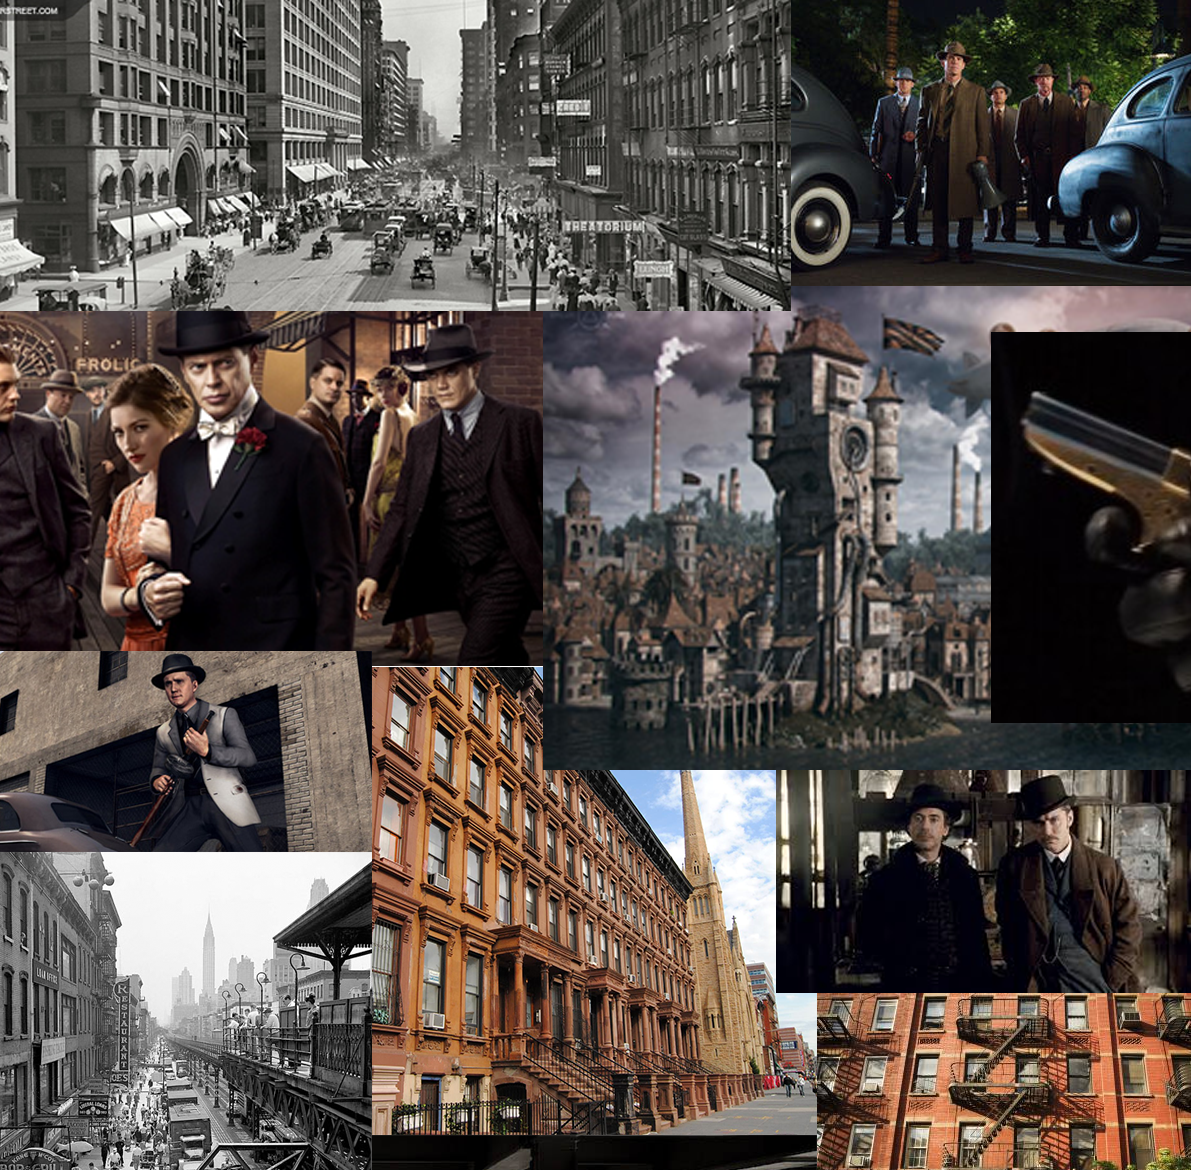
\includegraphics[width=120mm]{images/Collage.png}
		\end{figure}
	\subsection{Story and Main Characters}
		The game is based around a single story of a murder case. 
		\begin{quote}
			You are a businessman with a workaholic attitude, but a dark past. This is the day your past catches up to you. There is someone in your apartment. You try to run and escape from the madness that is now your reality. But it is to no avail.
		\end{quote}
		This is where our player comes in. As a detective, you have to collect evidence en ask people for information. With enough of it and we might even catch this bastard.
		\begin{quote}
			You are George Carter. A policeman, as clean as they come these days. There’s been a suicide, probably another overworked and coked up businessman again. It’s happening more often these days, since the economy went mad. It’s not been a happy couple of years, with your wife leaving and these suicides taking away all the joy. You go to the apartment. It’s a shabby old place, but nothing too bad. You’ve seen worse, much worse. The moment you get in something seems off. There is something that’s not as it seems.
		\end{quote}
		\noindent
		The game concludes in a finale, where, depending on the choices of the player, the killer is apprehended. The game is a sort of 'third person investigation' and is played by walking around in the scene with the arrow keys and collecting evidence by clicking on different objects to investigate them. In the end it will become clear who the killer is, if the player has gathered enough evidence. If the evidence collected is insufficient, the ending might not go as expected.\\ \\
\newpage

\section{Components}

\subsection{Procedural City, Rense}
In our game the city is generated procedurally every time you start up the game. But because the streets and landmarks are pre-set only all the houses are generated procedurally. In the city there are some large cubes which will become houses. The way it works is one script is dedicated to building smaller cubes from big cubes and gives them a tag what kind of house it is(left, right end and middle, both for if there is a house behind it or not). \\

	\begin{figure}[ht!]
		\centering
		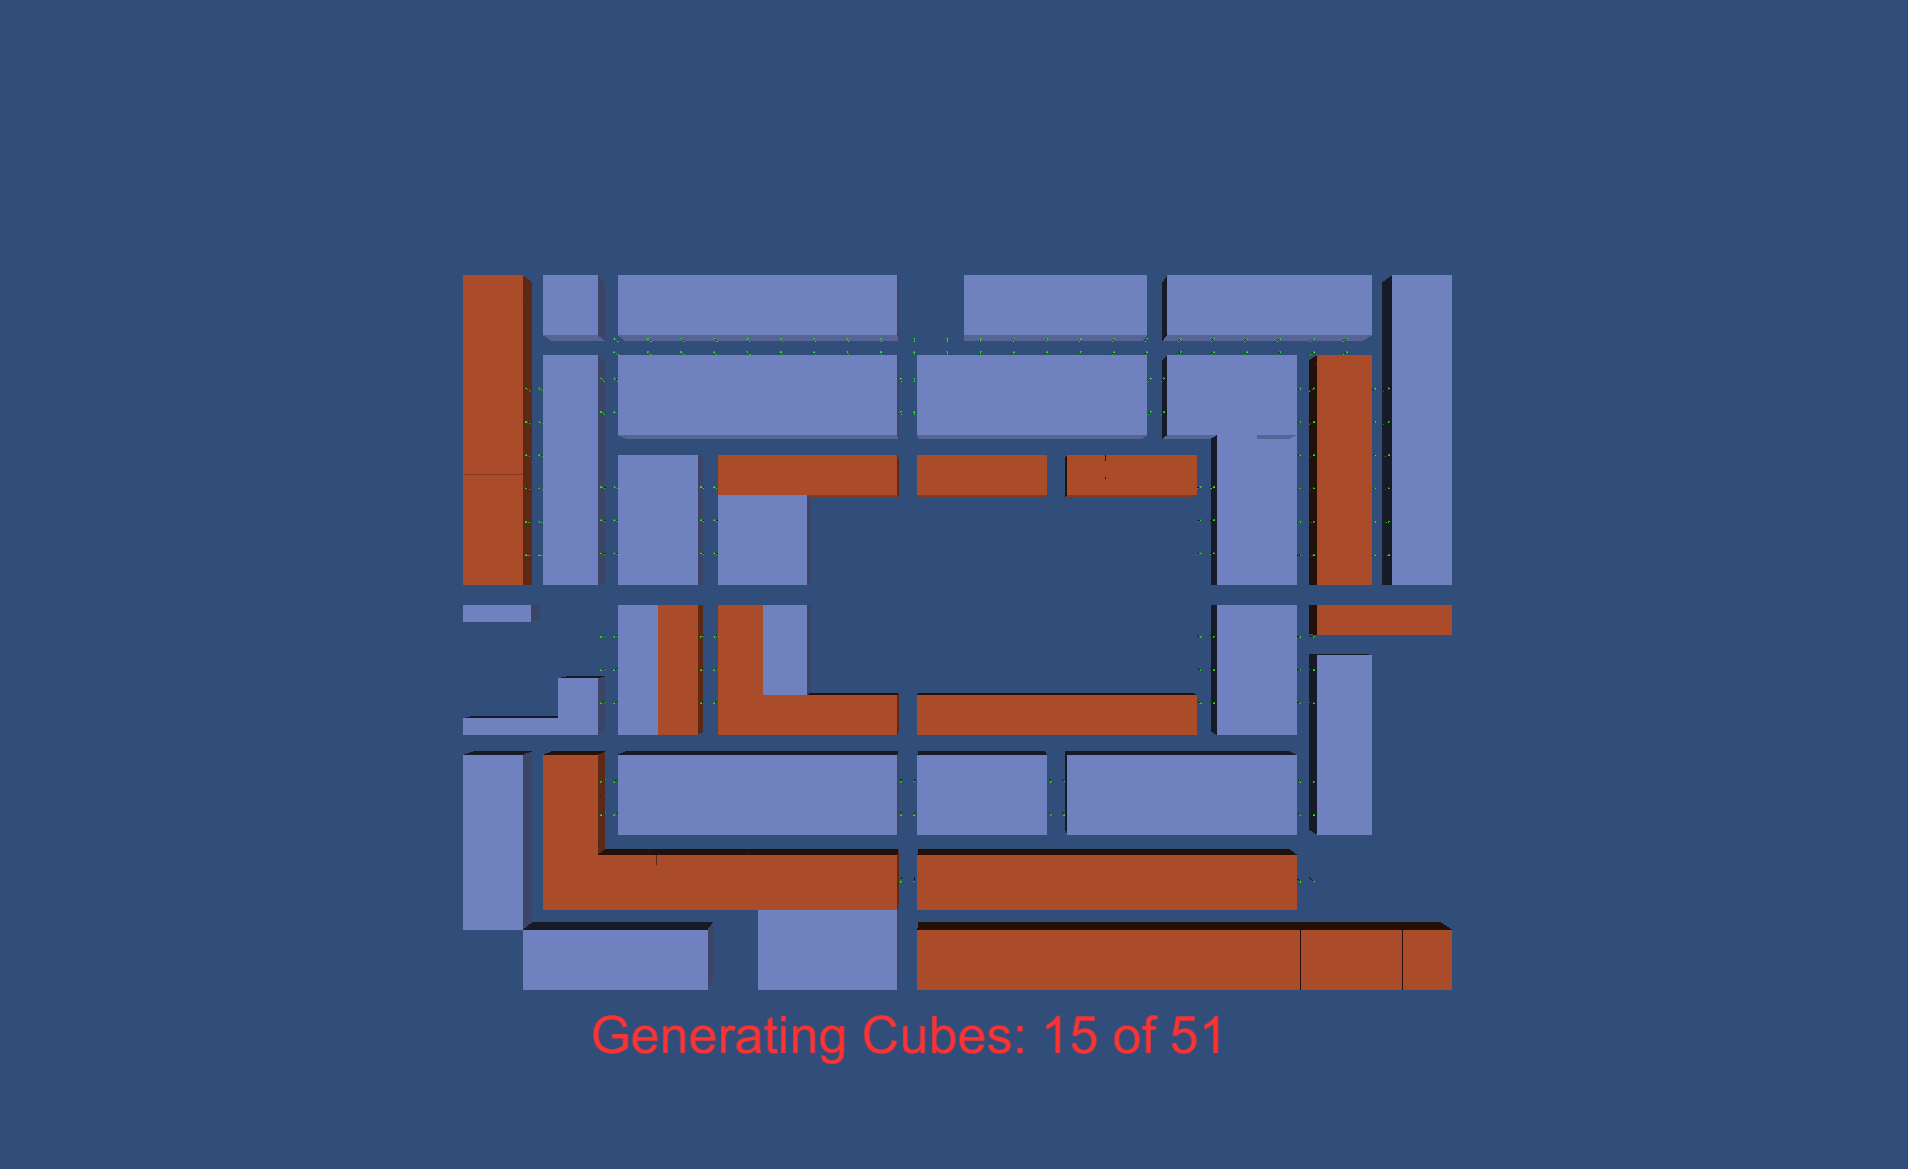
\includegraphics[width=70mm]{images/Procedural.png}
	\end{figure}
Then another script is dedicated to building houses from the smaller cubes, with a distinction between 6 kind of houses. From the smaller cube the house is made with a random depth, a random amount of windows and a random kind of roof(on a random rotation). If a house is at the end of the houseblok it also creates windows on the side. In the end every component of the house gets a random texture.\\



In the beginning this script took around 20 minutes to produce all the houses. But after some tweaking this is reduced to around 30 seconds to 1 minute. But still the houses are a big generator of lag due to setting it active and inactive between scenes.

	\begin{figure}[ht!]
		\centering
		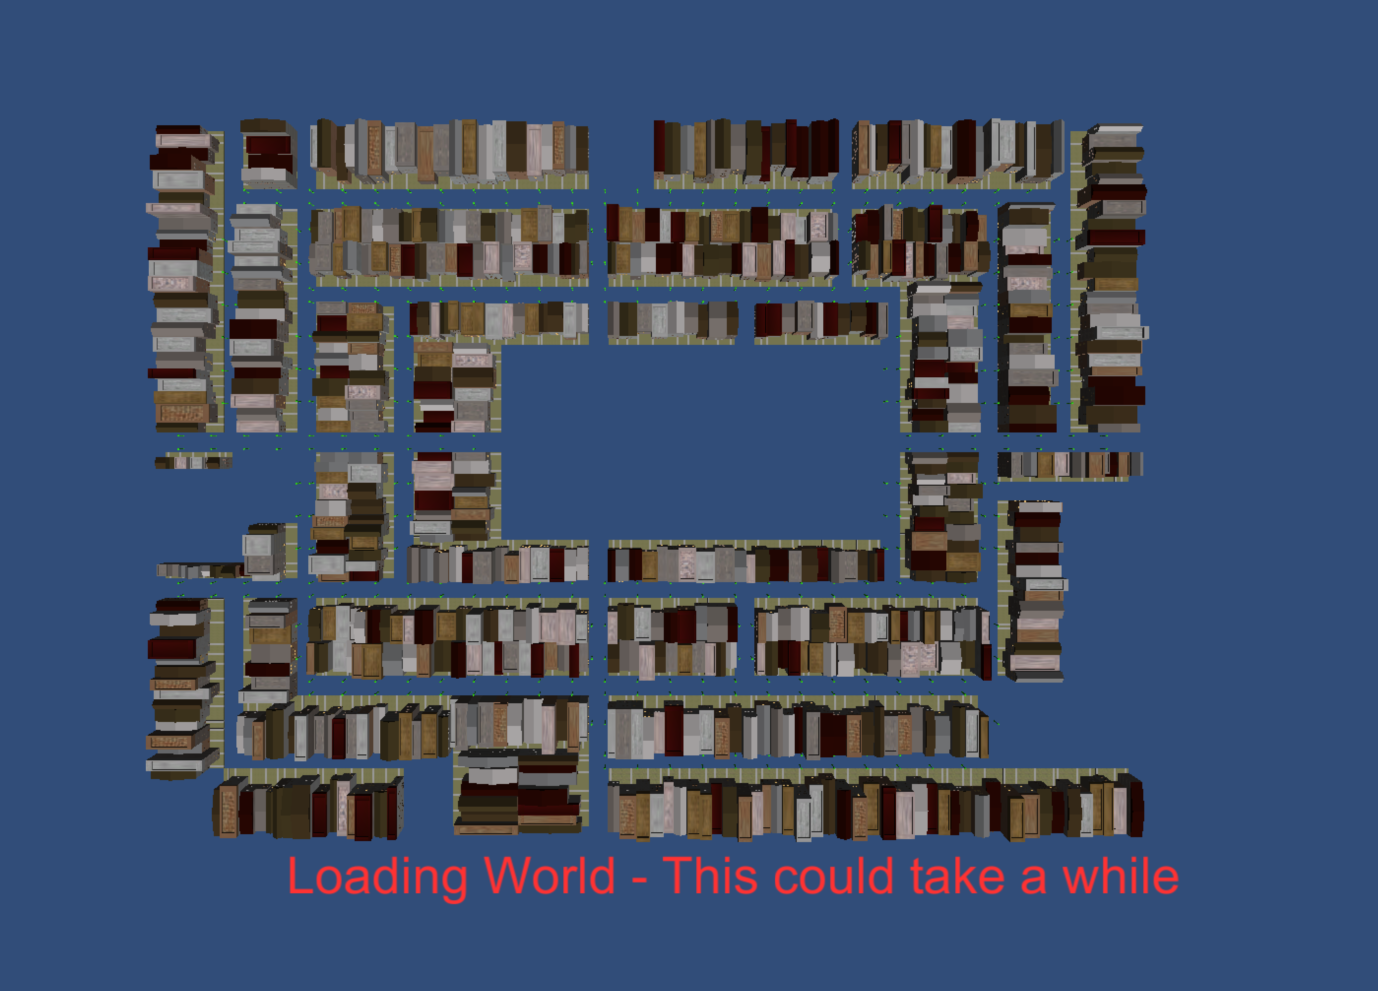
\includegraphics[width=70mm]{images/Generated.png}
	\end{figure}

	\newpage

\subsection{Navmesh, Jesper}
	To let cars drive autonomously through the city, a navmesh was created by Jesper. The most challenging part was to let cars keep driving on the right side of the road. In order to achieve this, the road was split up in parts: crossroads, lanes, line sections and dead ends. The dead ends were left out of the navmesh to avoid cars getting stuck at the end. A view of the navmesh can be seen in the figure below.

	\begin{figure}[ht!]
		\centering
		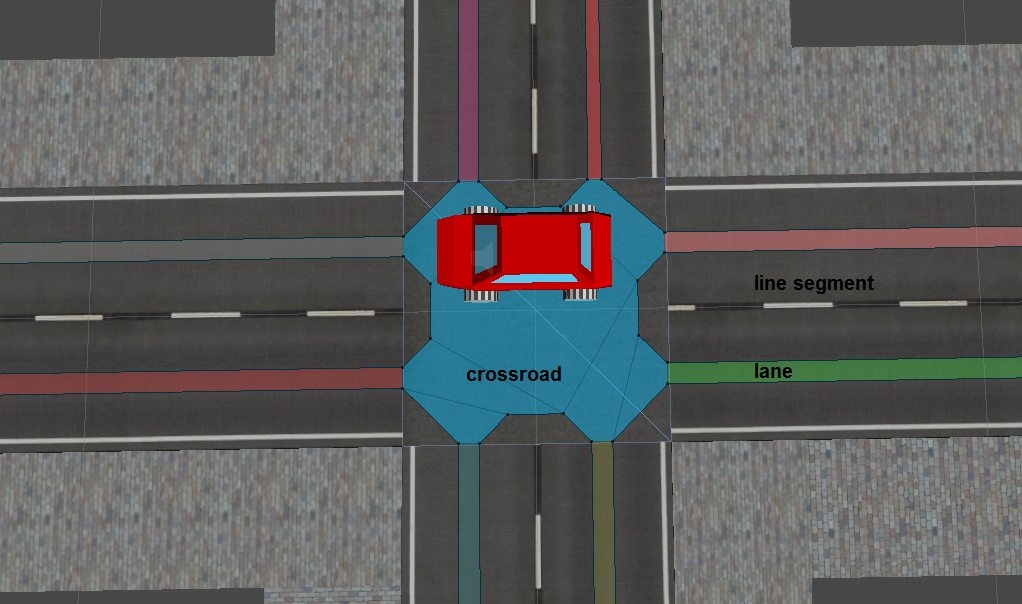
\includegraphics[width=120mm]{images/Navmesh.png}
	\end{figure}

	Because the path is calculated for the centre of the car and only the centre of the car stays on the navmesh, the lanes are narrow to avoid cars driving over the curb or the left lane. Every crossroad has its own index. All lanes to the left and below a certain crossroad have a lower index or the same and the lanes above and to the right have a higher index. When a car hits a crossroad, the costs for all lanes are again set to give all right sided lanes from that crossroad a low cost and all left sided roads a high cost. When a car gets within two units from its destination, a new destination is set and so the cars will keep driving around.

\subsection{A*, Boyd}
A  non-playable character (NPC) uses an A* pathfinding algorithm in our game. A* uses nodes to determine the route. Therefore a node network is created at the begin of the game. A node network is built out cube primitives. Each node is a trigger which determine whether the node is accessible. \\
The NPC chooses a random accessible node to walk to. Then the algorithm calculates the cost for each node. This is done by the taking the absolute distance and add an estimated distance value (the heuristic part) to this. After that A* determines which path has the lowest cost by taking the adjacent node with the lowest cost for each node.\\
The hardest part was making the node network  suitable for multiple NPCs. This was disregarded in the initial script. To solve this problem, the node keeps record of the costs for all NPCs in arrays.  The code had to be rewritten to accept this arrays.

\subsection{NPC Interaction, Boyd}
Our game needed a way to interact with NPCs. If clicked on an NPC with a mouse, an interface (new Unity UI) is activated. Then a script reads out an XML-file to determine the content of conversation. It is possible for NPCs to ask a question the player has to respond to. It depends on the answer of the player how the conversation continues. \\

	\begin{figure}[ht!]
		\centering
		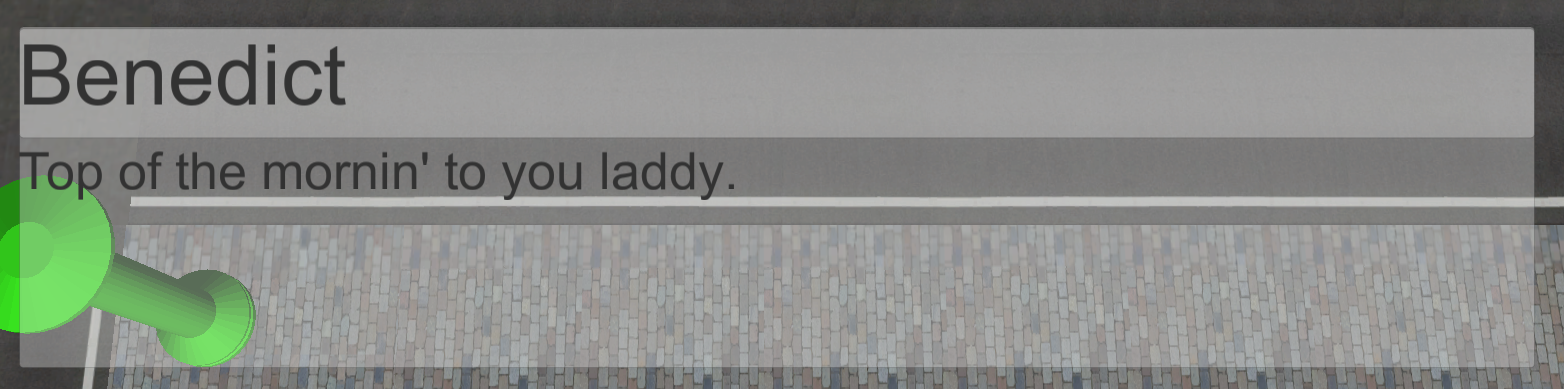
\includegraphics[width=120mm]{images/Conversation.png}
	\end{figure}

The major problem was making the conversation dependable on choices of the player. Therefore recursion was needed and this was difficult to implement. \\
Another problem was using the conversation interface if there were multiple NPCs in the scene. This was tackled by giving each NPC its own interface element. 



\subsection{Neural Network, Luuk}
In our game, we use a neural network to decide whether or not you catch the killer. The input for the network is a Boolean array with length nine. These Booleans represent pieces of evidence. The network consist of nine input neurons, ten hidden neurons and two output neurons, the two possible outcomes of the game. The network was trained in MatLab and the weights and thresholds were exported to Unity.\\
The training set was a set of 93 (19 percent of the total possible inputs) inputs with an output. This set was randomly divided in a training set and a test set. If the training set had 95\% correct, it goes to the test set. If that was 100\% correct, the network is considered trained. If that condition is not met, the network starts all over again with randomly dividing the sets. 

\subsection{Blender Rigging, Luuk}
Our character walks through the scenes with a walking animation. This character and the animation were created with blender. We first created a person in blender and tried to rig it. But the rigging failed, because the self-made model was too messy. To solve this, we used a human model from blendswap.com. Next we put clothes on the model and removed the skin from underneath the clothing. This was done because otherwise his arm would go through his shirt when he moved. The rigging was done with the rigify add-on in blender. With that rig, we made the walking animation that can be seen in the game.

	\begin{figure}[ht!]
		\centering
		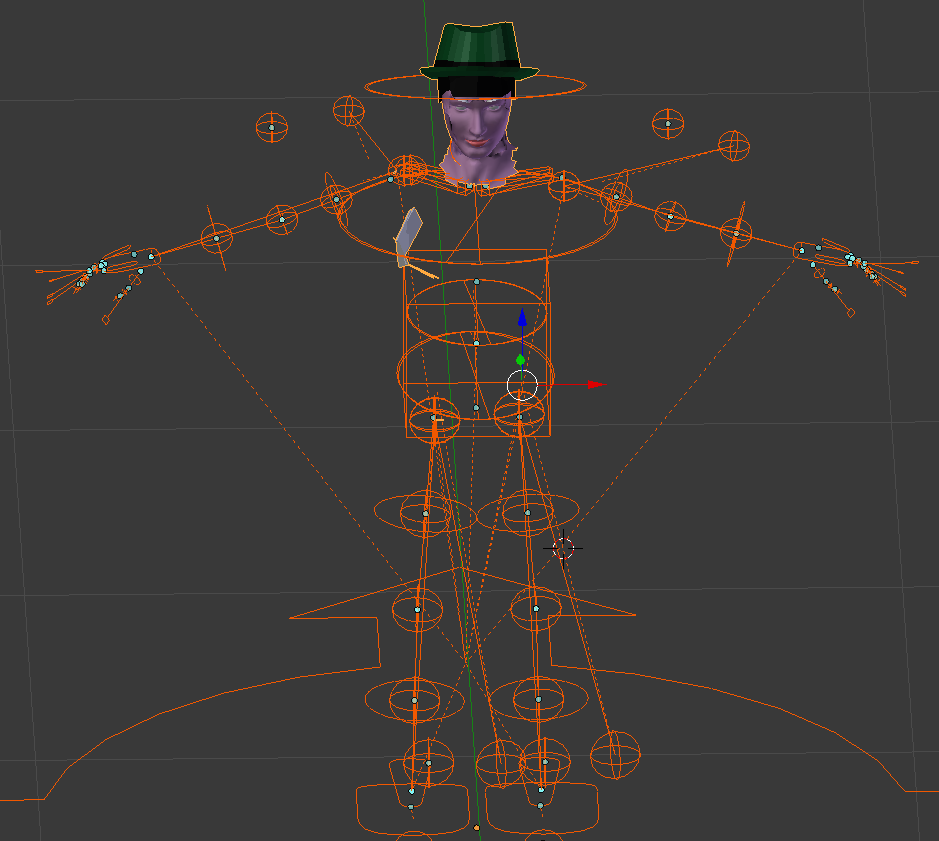
\includegraphics[width=70mm]{images/Rigging.png}
	\end{figure}

\subsection{Web \& Database, Thomas}
Awesome Spel uses a Web Server for some of its online features. The features mainly enable the player to keep track of their progress online, although offline play is possible. The following features come together to create our online save game platform:
\begin{itemize}
\item A secure user management system
\item Robust Server Side scripting with error reporting
\item MySQL database technology
\item Item and Location tracking
\end{itemize}
These features are implemented through the use of three individual modules:
\begin{enumerate}
\item A MySQL Database Server
\item Client Side Saved Game Management and Update calls
\item Server Side JavaScript to connect the two together.
\end{enumerate}
\subsubsection{The MySQL Database}
Our database uses modern, secure techniques of storing data. When an user is created, they are assigned an unique ID used to identify their actions and entries in the database. They receive an e-mail to Welcome them to the game and to give some general information. For secure storage of their passwords a pseudorandom 16-byte salt is generated that is then added to the password before hashing it with the Secure SHA256 hashing technique. Furthermore, every time the user logs in a new salt is generated and the password is rehashed to prevent the usage of rainbow tables even more. We use prepared statements to communicate with the database, to reduce the risk of SQL injection attacks. The database uses Indexes to make sure certain combinations of factors are always unique, for instance allowing the same player to only have any given item once. This further prevents any mishaps down the line.
\subsubsection{Client Side}
The client keeps track of a Saved Game file for storing the current player location and the items that are picked up. This Saved Game is also relayed to the server. When a player logs in the most recent data is acquired from the server. This is then written to the saved game, to allow local access and reduce the amount of requests the server has to process. Whenever the player enters a landmark or quits the game, their in-game location is send to the server. The same thing happens when a piece of evidence is picked up. The client side also allows players to create an account. The entered data are checked for formatting, such as e-mail addresses being valid and passwords matching client side. After that initial check the data, if valid, is relayed to the server where additional checks are run.
\subsubsection{Server Side}
The server uses JavaScript running on the Node.JS platform. We use the Express plugin to communicate with the client, although no static or dynamic content is actually served. We only transfer raw game data to and from the client. The server is built to keep running, which means we check our input and return errors is something is wrong, to both the client and the server logs. This can range anywhere from usernames already existing or passwords being incorrect, to incomplete or incorrect data being entered. Our system is the only system that provides a degree of security, as the permissions were set to enable ‘anyone’ to read data in the folders on the server by default, by the system administrator. We changed this to deny read access and protect our source code and the passwords inside it.

\newpage
\section{Code Quality}
Because multiple group members worked on the same scripts at different times, it was important to keep code clean organized and readable. This was done by separating code in functions as much as possible and leaving short comments as to what these functions were for. This made it possible for us to add to and change each other’s code. However, it did result in some problems. Sometimes code was dependent on other code, certain tags or other elements, which every now and then led into braking someone’s code by changing or adding something yourself. Luckily these errors were always easily fixed by looking over the code in question together.


\newpage
\section{Art}
\subsection{Models}
We made all the models in our game ourselves. Luuk worked on the evidence, the police station and the player model. This player model was replaced by a downloaded one at the last moment, because the rigging was not working properly. The downloaded player model is the only external model. Jesper made the landmarks, which were procedurally generated once and then stored, and world scene, with roads and the small parks. The rest of the buildings were procedurally generated by Rense, from unity. Thomas worked on the Church, the Hotel Room and the furniture in them. He also made the tree model.

	\begin{figure}[ht!]
		\centering
		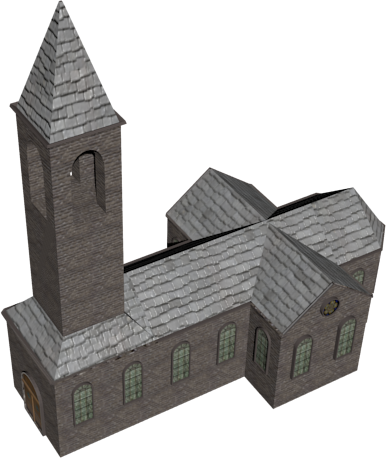
\includegraphics[width=60mm]{images/Churchoutside.png}
	\end{figure}

	\begin{figure}[ht!]
		\centering
		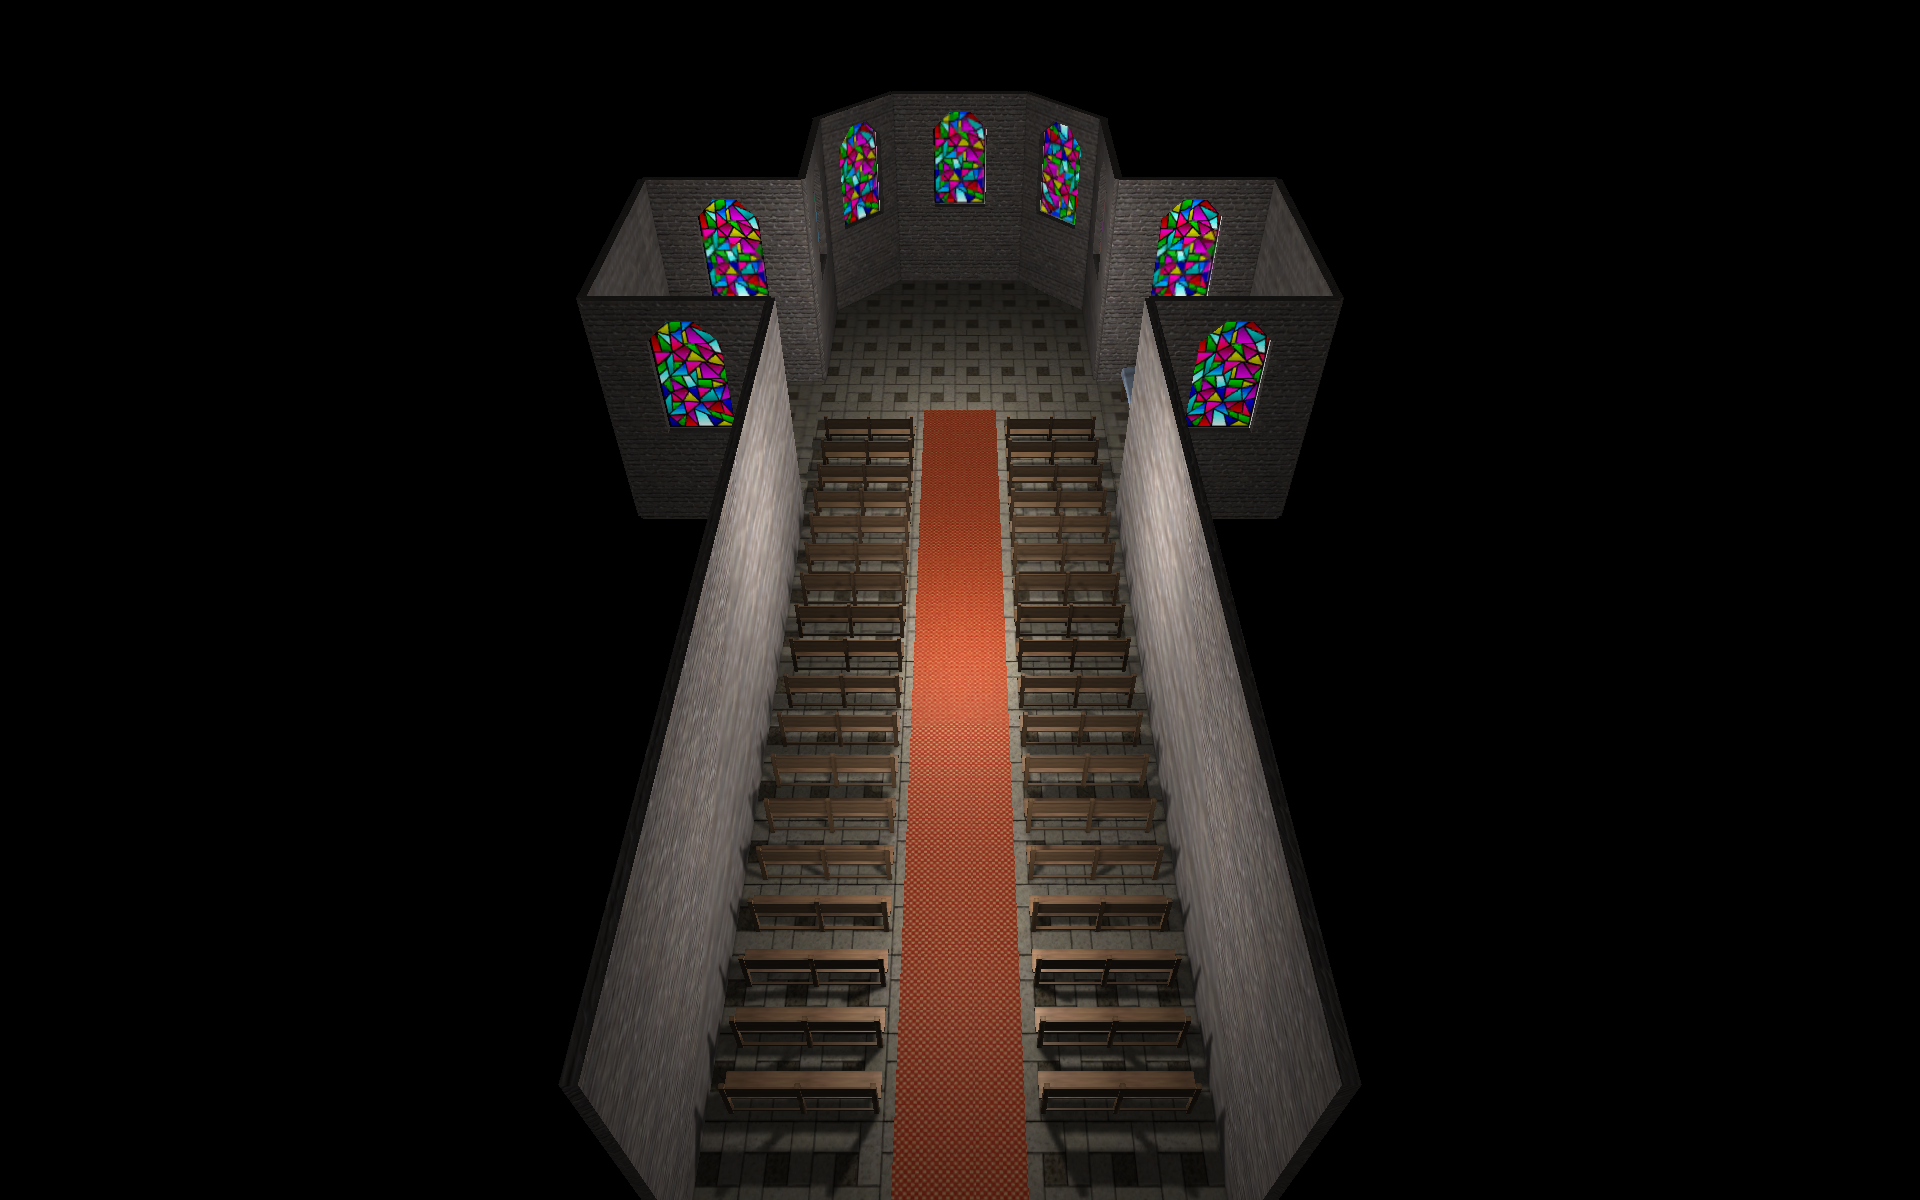
\includegraphics[width=90mm]{images/Church.png}
	\end{figure}



\subsection{Textures}
All the textures were downloaded externally from copyright free sources. All sources were credited within the game. Some textures were made seamless by us in Photoshop.

\subsection{Sound and Music}
The sounds were obtained from right free sources. They were edited to match the ambience better and sometimes to make them seamless by Thomas. The music was performed.


\newpage
\section{Process and Teamwork}
At the start of the process SCRUM was used extensively. Creating issues, assigning team members and setting a deadline cost a lot of time and therefor it was used less near the end of the process. It was also hard to decide when a component was finished. Most components were adapted many times up until the very end. As an addition to SCRUM we did always go over the issues that needed to be done at the beginning of every group session in a small discussion so everyone knew what to do that day. This also gave us a very regular update on how far we were in the process and if certain issues were harder than expected.\\

Working together as a team went great. We tried to always get together at the project sessions which helped a lot. Boyd and Rense as lead programmer and world builder respectively kept to their roles very well. The rest of the roles were not as clearly assigned to one person. Thomas, Luuk and Jesper all worked a lot in blender doing artistic things as well tackling more programming based issues as AI and web \& database components or creating parts of the world like the indoor scenes and the road system. Thomas also did most of his work as a game designer, including writing the game design document.\\

All in all the most important thing is that we did not have any issues working together. Everyone worked to his full potential and there was no weak link. This created a relaxed but driven atmosphere in the group.


\newpage
\section{Concluding}
At the start we had many ideas to make this a great game. Looking back on it, we were a little bit too ambitious which means the result is not exactly as we had in mind. Because it was important to create challenging components in the game, we had to cut down on some of the gameplay aspects. This means that it is not as an exciting game as we were going for. In retrospect we should have probably chosen a game with an easier game design, giving us more time to focus on the gameplay and the juiciness. We were very happy with the teamwork. The one thing that we would improve for a next game is improving our knowledge of all the programs before starting to build the game. This would save us from redoing the same thing over and over again. (But I guess that is part of the job)
In conclusion we are very happy with the end result. All the components are there. We just needed a little more time to make it into a juicy exciting game.



\end{document}